% !TeX root = Report.tex
\documentclass[12pt]{article}

% Package imports (organized and deduplicated)
\usepackage{biblatex}
\usepackage{changepage}
\usepackage{color}
\usepackage{enumitem}
\usepackage{float}
\usepackage{graphicx}
\usepackage{listings}
\usepackage{sectsty}
\usepackage{xcolor}
\usepackage[breaklinks=true]{hyperref}
\usepackage{xurl}
\usepackage{tikz}
\usepackage{tabularx}
\usetikzlibrary{shapes.geometric,positioning,fit,backgrounds}
\usepackage{./timing-diagrams}
\usetikzlibrary{calc}
\setcounter{biburlnumpenalty}{100}
\setcounter{biburlucpenalty}{100}
\setcounter{biburllcpenalty}{100}

\definecolor{darkblue}{RGB}{0, 0, 102} 
\hypersetup{
    colorlinks=true,
    pdfborder={0 0 0},
    linkbordercolor=white,
    urlcolor=darkblue,
    linkcolor=darkblue,
    citecolor=darkblue,
    filecolor=darkblue
}

% Make bibliography ragged right instead of justified
\AtBeginDocument{
  \renewcommand{\bibsetup}{\raggedright}
}
% Document configuration
\restylefloat{table}
\graphicspath{{./images/}}
\addbibresource{Library.bib}
\subsectionfont{\fontsize{12}{14}\selectfont}

% Author information
\author{
    Joar Heimonen\\
    \texttt{contact@joar.me}
}

% Title configuration
\title{
    \textbf{PEAK}\\[0.5em]
    \large \textbf{P}roxy \textbf{E}liminating \textbf{A}rchitecture using \textbf{K}ubernetes\\[0.3em]
    \large A research propsal
}
\date{\today}

\newcommand{\license}{
    \vspace{1em}
    \noindent\small{© 2025 Joar Heimonen\\
    This work is licensed under a \href{https://creativecommons.org/licenses/by-sa/4.0/}{Creative Commons Attribution-Sharealike 4.0 International License}.}
    \vspace{1em}
}

\begin{document}
\maketitle

\pagebreak

\tableofcontents

\pagebreak


\section{Part 1}
\subsection{Introduction}
With the adoption of IPv6 \cite{hindenInternetProtocolVersion1998a} our networking landscape is about to change. Last year we proposed the architecture \textbf{PEAK} \cite{heimonenPreprintPEAKProxy2024} which leverages the new capabilities of IPv6
to create distributed systems that are not reliant on proxies.
Our last paper introduced a reference implementation of the PEAK architecture, while this is useful it does not allow us to benchmark and compare the performance of 
the PEAK architecture to traditional systems.
\\
\\
While the PEAK article \cite{heimonenPreprintPEAKProxy2024} was a qualitative study, this paper proposes a quantitative study of the PEAK architecture.
This quantitative study will be performed according to the guidelines set forth by "Research Design: Qualitative, Quantitative, and Mixed Methods Approaches" \cite{creswellResearchDesignQualitative}.
We will However not be performing a Mixed Methods study as this all ready has been done in the PEAK article \cite{heimonenPreprintPEAKProxy2024}.
\\
\\
In this paper we propose a set of reference implementations of the PEAK architecture that will be benchmarked against a set of traditional systems.
We will also propose a set of metrics that will be used to compare the performance of the systems.
With the aim of showing that the PEAK architecture not only is viable but matches or exceeds the performance of traditional systems.
We hope that the data driven approach of this paper will help to further the adoption of the PEAK architecture.

\subsection{Background}
Since the start of this century, the internet has grown from a small network of universities to a global network that connects billions of devices. Due to our limited
address space provided by IPv4 \cite{InternetProtocol1981} we have not been able to give every device a unique address. This has led to the development of two technologies. Network address translation (NAT) \cite{holdregeIPNetworkAddress1999} and proxies.
\\
\\
NAT allows for the creation of subnets that can be used to connect multiple devices to the internet through a single shared IP address. This is a great solution for small networks
but leads to an increase in complexity as the network grows. In a subnet consisting of servers none of these servers can be reached from the internet without the use of a proxy.
The proxy simply redirects traffic to the correct server in the subnet based on arbitrary rules.
\\
\\
While proxies works fine they introduce a single point of failure in distributed systems. If the proxy stops working, all the servers within the subnet become unreachable.

\section{Part 2}
\subsection{Relevant Work}
As mentioned in the PEAK article \cite{heimonenPreprintPEAKProxy2024} distributed systems with DNS for load balancing and routing is not a new concept.
However, it has proven to be a challenge to find recent research on the topic.
\\
\\
\textit{Table 1} shows the search terms we used and the results from these searches. As can be seen
there is a lack of research on the topic. Our exclusion parameters were set to exclude any research older than 2020.
We also excluded any research that did not mention DNS, load balancing and distributed systems in the abstract.

\begin{table}[H]
    \centering
    \begin{tabularx}{\textwidth}{|l|X|c|c|c|}
        \hline
        \textbf{DB} & \textbf{Keywords} & \textbf{Date} & \textbf{Res.} & \textbf{Rel.} \\
        \hline
        IEEE & Dist. Sys. AND DNS & 17-Feb-25 & 117 & 0 \\
        \hline
        IEEE & Load bal. AND DNS & 17-Feb-25 & 33 & 0 \\
        \hline
        IEEE & Dist. Sys. AND Load bal. AND DNS & 17-Feb-25 & 13 & 0 \\
        \hline
        Google Scholar* & CERN AND Load bal. AND DNS & 17-Feb-25 & 40 & 2 \\
        \hline
        ACM & Dist. Sys. AND DNS & 18-Feb-25 & 388 & 0 \\
        \hline
        ACM & Load bal. AND DNS & 18-Feb-25 & 161 & 0 \\
        \hline
        ACM & Dist. Sys. AND Load bal. AND DNS & 18-Feb-25 & 154 & 0 \\
        \hline
    \end{tabularx}
    \caption{Search results \textit{*Google Scholar is a meta-database, The results are from the first four pages.}}
\end{table}

Due to the lack of search results we quickly realized that it would be beneficial to use a meta-database such as Google Scholar.
This gave us two relevant articles from CERN.

\newpage

\noindent\rule{\textwidth}{0.4pt}
\begin{itemize}
    \item \textbf{Title:} Achieving metric oriented load balancing \cite{canilhoAchievingMetricOriented2020}
    \item \textbf{Authors:} P. Canilho, I. Reguero, P. Saiz
    \item \textbf{Date:} 2020
    \item \textbf{Data:} "This article presented the objectives, advantages and usage of a metric-based load balancing solution that is actively maintained at CERN." \cite{canilhoAchievingMetricOriented2020}
    \item \textbf{Methods:} Theoretical Paper
    \item \textbf{Main Findings*:} Implemented metric-based load balancing through SNMP and their own lbclient. Does not mention how this can be applied to the larger IPv6 space.
\end{itemize}
\noindent\rule{\textwidth}{0.4pt}
\begin{itemize}
    \item \textbf{Title:} A Modernized Architecture for the Post Mortem System at CERN \cite{barthModernizedArchitecturePost2022}
    \item \textbf{Authors:} J. Barth, F. Bogyai, J. Garnier, M. Majewski, T. Martins Riberio, A. Mnich, M. Pocwierz, R. Selvek, R. Simpsons, A. Stanisz, D. Wollmann, M. Zerlauth
    \item \textbf{Date:} 2022
    \item \textbf{Data:} Redesign of the post mortem system at the large hadron collider \cite{barthModernizedArchitecturePost2022}.
    \item \textbf{Methods:} Theoretical Paper
    \item \textbf{Main Findings*:} Implemented load balancing trough DNS to make the post mortem system of the large hadron collider horizontally scalable.
\end{itemize}
\noindent\rule{\textwidth}{0.4pt}
\textbf{*Main findings in relation to the PEAK architecture \cite{heimonenPreprintPEAKProxy2024}.}

\subsection{Initial Analysis}
We were able to find two articles that address routing trough DNS and metric based load balancing \cite{heimonenPreprintPEAKProxy2024,canilhoAchievingMetricOriented2020}. 
However, none of these articles mention the use of IPv6 to create a public distributed system that is not reliant on proxies.
Neither of the articles perform any form of benchmarking to compare the performance of their systems to more traditional systems. 
Due to the lack of research on this topic we believe that we have found a gap in research on the topic of modern distributed systems.
While it is somewhat disconcerting that we were not able to find more research on the topic, we are 
also presented with an exciting opportunity to further the field of distributed systems.
This further demonstrates the need for a quantitative study of not only the PEAK architecture but also
more conventional systems.
\\
\\
As a system grows in complexity qualitative studies \cite{creswellResearchDesignQualitative} become more and more disconnected from the reality of the system.
This is why we believe that a quantitative study is needed to further the field of distributed systems.


\section{Part 3}
\subsection{Research Questions}
We aim to answer the following questions:
\begin{enumerate}
    \item How does the PEAK architecture perform compared to traditional systems?
    \item What metrics can be used to compare the performance of the PEAK architecture to traditional systems?
    \item How does the PEAK architecture scale compared to traditional systems?
\end{enumerate}
To achieve this goal this paper will propose a set of reference implementations of the PEAK architecture and a set of traditional counterparts.
We will also propose a set of metrics that can be used to compare the performance of the systems.

\subsection{Reference Implementations}
We propose the following two reference implementations and their traditional counterparts:

\subsubsection{Reference Implementation 1}
This reference implementation consists of a set of servers where routing and load balancing is handled through the cluster level DNS server.
This can be seen in \textit{Figure \ref{fig:test-one}}.

\begin{figure}[H]
    \centering
    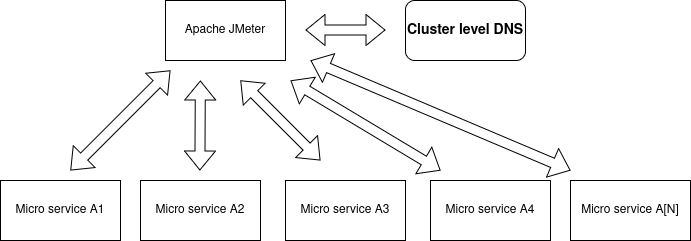
\includegraphics[width=\textwidth]{test-one.drawio.png}
    \caption{PEAK reference implementation 1}
    \label{fig:test-one}
\end{figure}

A counterpart to this reference implementation consists of a proxy server that routes traffic to the servers. This can be seen in \textit{Figure \ref{fig:test-one-traditional}}.

\begin{figure}[H]
    \centering
    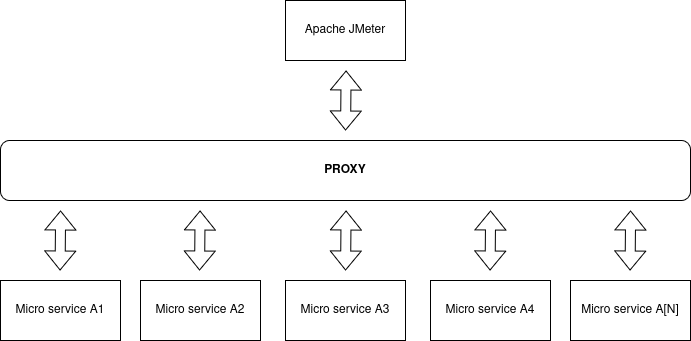
\includegraphics[width=\textwidth]{test-one-traditional.drawio.png}
    \caption{Reference implementation 1 traditional counterpart}
    \label{fig:test-one-traditional}
\end{figure}

\subsubsection{Reference Implementation 2}
This reference implementation is designed to test the client-mediated communication suggested in the PEAK architecture \cite{heimonenPreprintPEAKProxy2024}.
This can be seen in \textit{Figure \ref{fig:test-two}}.

\begin{figure}[H]
    \centering
    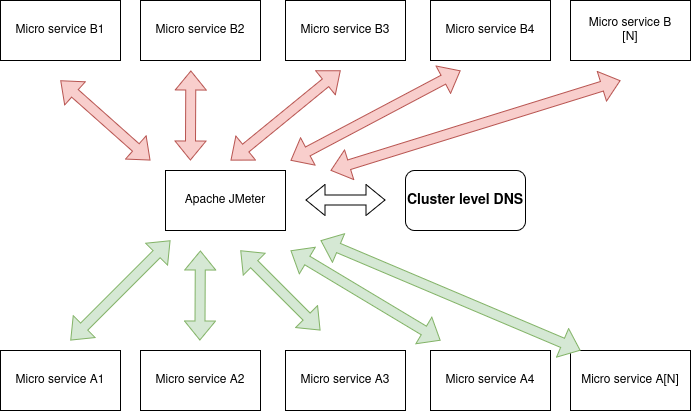
\includegraphics[width=\textwidth]{test-two.drawio.png}
    \caption{PEAK reference implementation 2. The green arrows represent request 1 and the red arrows represent request 2.
    The A set of servers signs a token that must be presented to the B set of servers to be able to communicate.}
    \label{fig:test-two}
\end{figure}

A counterpart to this reference implementation that replaces the client mediated communication with a service mesh can be seen in \textit{Figure \ref{fig:test-two-traditional}}.

\begin{figure}[H]
    \centering
    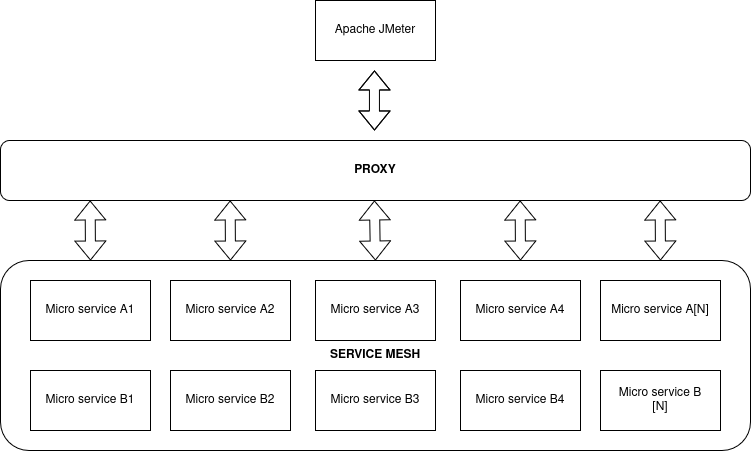
\includegraphics[width=\textwidth]{test-two-traditional.drawio.png}
    \caption{Reference implementation 2 traditional counterpart}
    \label{fig:test-two-traditional}
\end{figure}

\subsection{Metrics}
There are six metrics that we can use to compare the performance of the PEAK architecture to traditional systems:
\begin{enumerate}
    \item \textbf{Latency:} The time it takes for a request to be processed.
    \item \textbf{Throughput:} The number of requests that can be processed in a given time frame.
    \item \textbf{Scalability:} How well the system scales as the number of servers increases.
    \item \textbf{Balance:} How well the system balances the load between the servers.
    \item \textbf{Inner service communication:} How well the system handles communication between servers.
    \item \textbf{Fault tolerance:} How well the system handles server failures.
\end{enumerate}
There are also several combinations of these metrics that can be used to compare the performance of the systems.
Like the ratio between throughput and Scalability. In a perfect system we expect the throughput to increase linearly as the number of servers increases.
Latency and Scalability can also be combined to see how the latency increases as the number of servers increases. 

\subsection{Methodology}
The reference implementations will be implemented in a Kubernetes cluster.
The cluster will contain a single cluster level DNS server \cite{heimonenPreprintPEAKProxy2024} or a single proxy server.
We will ramp up Apache JMeter \cite{ApacheJMeterApache} until the system fails. 
After the system has failed we will increase the number of servers and try again.
This will be done for both the PEAK architecture and the traditional systems.
A flow diagram of the testing process can be seen in \textit{Figure \ref{fig:flow-chart}}.
The results will be compared using the metrics proposed in the previous section through a comparative analysis.
\\
\\
\begin{figure}[H]
    \centering
    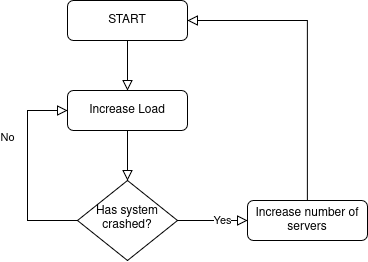
\includegraphics[width=0.7\textwidth]{flow chart.drawio.png}
    \caption{A flow chart of the testing process. 
    This test runs until the desired number of servers has been reached.}
    \label{fig:flow-chart}
\end{figure}

\section{Part 4}
\subsection{Discussion}
While our approach to quantitative testing \cite{creswellResearchDesignQualitative} seems simple enough on paper.
It is worth remembering that there are hundreds of configurations not only for the PEAK architecture but also for the traditional systems
that can be tested. It is essential that both of the systems are created in an as efficient and lean way as possible.
This helps to mitigate the risk of a system underperforming due to a misconfiguration.
A potential solution to this problem is outsourcing the creation of the traditional systems to multiple parties.
Multiple implementations of the traditional system created by different parties will strengthen the validity of the results
by guaranteeing that the traditional systems are created in an impartial manner.
\\
\\
Providing that the proposed quantitative study is performed correctly, we believe that this work 
has the potential to disrupt the status quo of distributed systems. Resulting in less bloated
systems that are more fault-tolerant and scalable. We also hope that this work will inspire others 
to further the field of distributed systems with original ideas and architectures.



\addcontentsline{toc}{section}{References}
\printbibliography
\license
\end{document}